\documentclass[11pt]{article}

\usepackage{times}
\usepackage{geometry}
\usepackage{float}
\geometry{margin=1in}
\usepackage{amsmath,amssymb}
\usepackage{booktabs}
\usepackage{graphicx}
\usepackage{url}
\usepackage{hyperref}
\usepackage{placeins}
\usepackage{appendix}
\usepackage[ruled,vlined]{algorithm2e}
\SetKw{KwState}{State}
\renewcommand{\appendixname}{Appendix}
\usepackage[final]{microtype}

\title{\bf When F1 Fails: Granularity-Aware Evaluation for Dialogue Topic Segmentation}

\author{
Michael H. Coen\\
Independent Researcher\\
mhcoen@alum.mit.edu
}

\date{Preprint. Under review.}

\begin{document}
\maketitle

\begin{abstract}
Dialogue topic segmentation supports summarization, retrieval, memory
management, and conversational continuity. Despite decades of prior
work, evaluation practice in dialogue topic segmentation remains
dominated by strict boundary matching and F1-based
metrics~\cite{vanrijsbergen1979,liu2024dialogseg}, even as modern
LLM-based conversational systems increasingly rely on segmentation to
manage conversation history beyond the model's fixed context window,
where unstructured context accumulation degrades efficiency and
coherence.

This paper introduces an evaluation objective for dialogue topic
segmentation that treats boundary density and segment coherence as
primary criteria, alongside window-tolerant F1 (W-F1). Through
cross-dataset empirical evaluation, we show that reported performance
differences across dialogue segmentation benchmarks are driven not by
model quality, but by annotation granularity mismatches and sparse
boundary labels. This indicates that many reported improvements arise
from evaluation artifacts rather than improved boundary
detection. Moreover, across these benchmarks, variation in boundary
density (BOR) explains substantially more variation in F1/W-F1 than
differences between segmentation methods, even when using a stronger
neural boundary scorer.

We evaluated multiple, structurally distinct dialogue segmentation
strategies across eight dialogue datasets spanning task-oriented,
open-domain, meeting-style, and synthetic interactions. Across these
settings, we observe high segment coherence combined with extreme
oversegmentation relative to sparse labels, producing misleadingly low
exact-match F1 scores. We show that topic segmentation is best
understood as selecting an appropriate granularity rather than
predicting a single correct boundary set. We operationalize this view
by explicitly separating boundary scoring from boundary selection.
\end{abstract}

\section{Introduction}
Dialogue topic segmentation is commonly framed as identifying points
in a conversation where ``the subject changes.'' This framing is
appealingly simple. It is also incorrect. Topic structure is often
gradual, nested, and perspective-dependent.

Despite this, many dialogue segmentation benchmarks treat annotated
boundaries as objective ground truth and evaluate systems using strict
boundary matching and F1-based metrics~\cite{vanrijsbergen1979}. These
metrics collapse distinct failure modes into a single number. Small
boundary shifts are often harmless when the goal is coherent topic
blocks, while missing or adding a few boundaries can be catastrophic
if boundaries drive downstream actions such as summarizing or dropping
earlier turns.

This paper addresses that mismatch by reframing what gets reported and
what gets optimized. The evaluation objective in this paper jointly
reports (i) window-tolerant F1 (W-F1), (ii) boundary density, and
(iii) segment coherence. An accompanying algorithmic contribution
separates boundary scoring from boundary selection, making boundary
density explicit and controllable. Together, these contributions
distinguish detection failures from granularity mismatches (i.e.,
discrepancies between the segmentation resolution at which boundaries
are produced and that implied by the annotation scheme) and explain
why a single global threshold fails to transfer across
datasets.

We distinguish between two notions that are often conflated in
boundary-based evaluation.  \emph{Boundary placement alignment} refers
to whether predicted boundaries occur at the same locations as gold
boundaries (within a tolerance window), which is the intended target
of metrics such as F1 and W-F1.  By contrast, \emph{boundary density
alignment} refers only to whether the number of predicted boundaries
matches the number implied by the annotation scheme, independent of
where those boundaries are placed.  \emph{Segmentation granularity} is
a modeling and selection-level property that determines boundary
density through the boundary selection rule, sometimes implicitly, and
thereby strongly influences boundary-based metrics.

It bears emphasizing that boundary-based metrics such as F1 remain
appropriate when annotation granularity is consistent between
training, evaluation, and intended use. The failure modes illustrated
here arise when segmentation granularity differs across datasets or
between system behavior and annotation intent---an increasingly common
situation in dialogue benchmarks and downstream applications.

This paper does not propose a new segmentation model. The contribution
is an evaluation perspective and a principled separation between
boundary scoring and boundary selection that exposes granularity
effects obscured by standard metrics. Concretely, the contributions
are as follows:

\begin{itemize}
\item We show that boundary-based metrics (including F1 and W-F1) can
  be dominated by boundary density alignment: even non-semantic
  baselines achieve competitive scores when their output density
  matches the gold annotation.
\item We propose a composite evaluation objective that reports
  boundary density and segment coherence alongside W-F1, exposing
  failure modes hidden by standard boundary metrics.
\item A two-stage topic segmentation framework is introduced and
  empirically validated that separates boundary scoring from boundary
  selection, making boundary density an explicit design choice rather
  than an accidental side effect of threshold tuning.
\end{itemize}

Standard boundary-based evaluation implicitly assumes that, once boundary density is controlled,
differences in F1 or W-F1 primarily reflect differences in boundary placement quality rather than
thresholding or selection behavior.
A central empirical finding of this work is that boundary-based evaluation metrics are dominated
by segmentation granularity induced by boundary selection, rather than by boundary detection quality.
In particular, for a fixed scoring model, sweeping the boundary selection threshold produces larger
changes in W-F1 than switching between structurally distinct segmentation methods, a pattern made
explicit by density--quality curves in Section~\ref{sec:results}
(Figure~\ref{fig:density-quality}).
As a result, leaderboard-style comparisons that report only a single operating point can conflate
method improvements with shifts in boundary density.

\subsection{Motivation: Conversational Memory in AI Chat Systems}

Large language model (LLM) based chat systems operate under finite context
windows, which require practical systems to manage conversational history
explicitly. As conversations grow longer, earlier turns must be dropped,
summarized, or selectively retrieved. Topic segmentation decisions therefore
directly determine which portions of prior dialogue are preserved, compressed,
or reintroduced.

Importantly, this challenge does not disappear as context windows grow larger.
Unstructured accumulation of earlier dialogue increases computational cost and
dilutes relevance, reducing the model's ability to focus on salient information.
Effective conversational systems therefore require explicit structure over
dialogue history rather than unbounded context expansion.

In this setting, topic segmentation functions as a memory control mechanism
rather than a purely linguistic task. Poor segmentation can cause relevant
context to be discarded prematurely or irrelevant context to be retained,
leading to degraded long-horizon coherence and unstable behavior across turns.
The absence of robust episodic memory remains a major limitation of current
LLM-based systems, particularly in multi-session interactions.

This work is motivated by the development of \emph{Episodic}, a
conversational memory system that organizes dialogue into
topic-structured representations to support persistent interactions
with LLM-based assistants~\cite{episodic_github}.  Within such
systems, boundary placement governs summarization, retrieval, and
context reintegration, making segmentation granularity a first-order
systems design decision rather than an evaluation detail.


\section{Background and Related Work}

Topic segmentation has a long history in text processing, with
evaluation practice, dataset design, and granularity assumptions
evolving somewhat independently. We organize prior work along these
three dimensions.

\subsection{Boundary-Based Evaluation Metrics}
Topic segmentation evaluation has historically centered on boundary
alignment. Early metrics such as Pk~\cite{beeferman1999statistical} penalized
segmentations where predicted and gold boundaries fell in different
segments under a sliding window. WindowDiff~\cite{pevzner2002critique} refined
this approach to address Pk's known biases. Both metrics assume a
single correct segmentation and measure deviation from it.  More
recent dialogue segmentation work has largely adopted precision,
recall, and exact-match F1 computed over boundary
positions~\cite{vanrijsbergen1979, liu2024dialogseg}. These metrics
inherit the same assumption: that annotated boundaries represent
ground truth rather than one valid segmentation among many. When
annotation granularity varies across datasets or differs from system
behavior, this assumption produces misleading evaluations.

\subsection{Dialogue Segmentation Datasets}
Dialogue topic segmentation introduces complexity beyond written text
due to turn-taking, discourse phenomena, and ill-defined topic
boundaries. Several benchmarks have emerged with distinct annotation
philosophies. DialSeg711~\cite{dialseg711} and
SuperDialseg~\cite{superdialseg2023} provide densely annotated
dialogue corpora, while TIAGE~\cite{tiage} annotates topic
boundaries in task-oriented dialogue with sparser labels tied to task
structure. MultiWOZ~\cite{budzianowski2018multiwoz} provides domain
annotations that can be interpreted as coarse topic boundaries.
Open-domain and semi-structured datasets such as
DailyDialog~\cite{li2020dailydialog}, Taskmaster~\cite{byrne2019taskmaster}, 
Topical-Chat~\cite{topicalchat}, and QMSum~\cite{zhong2021qmsum} reflect
further variation in annotation intent, from synthetic concatenation
boundaries to summarization-driven segmentation. This diversity in
annotation philosophy produces systematic differences in boundary
density across datasets—differences that standard metrics do not
distinguish from detection quality.

\subsection{Segmentation Granularity}
Classic segmentation methods such as
TextTiling~\cite{hearst1997texttiling}
and Choi-style
benchmarks~\cite{choi2000advances} established the paradigm of predicting a
single boundary set evaluated against gold annotations. Subsequent
work has refined scoring models and architectures, but the assumption
that a single correct granularity exists has remained largely
unexamined.  Prior work rarely treats segmentation granularity as a
first-class, controllable variable. Boundary density is typically a
side effect of threshold tuning rather than an explicit design choice,
and evaluation protocols do not distinguish between detection failures
(placing boundaries at wrong locations) and granularity mismatches
(producing a different number of boundaries than the annotation scheme
implies). This paper addresses that gap by separating boundary scoring
from boundary selection and proposing evaluation criteria that make
granularity effects explicit.


\section{Problem Setting}
\label{sec:problem-setting}
Topic boundaries are not intrinsic properties of conversations. They
depend on segmentation granularity induced by boundary selection, task
requirements, and annotation intent. A model that produces
fine-grained discourse-phase boundaries can be operationally
reasonable yet score poorly against a dataset that annotates only
coarse task transitions. Conversely, a model tuned to sparse labels
can suppress meaningful structure. Figure~\ref{fig:worked_example}
provides a concrete worked example illustrating this failure mode.

This paper treats topic segmentation as two separate operations:
\begin{enumerate}
\item \textbf{Boundary scoring:} assign a score to each candidate
  boundary position.
\item \textbf{Boundary selection:} choose which candidates become
  output boundaries, controlling boundary density and spacing.
\end{enumerate}

Collapsing these operations makes boundary density an accidental
byproduct of threshold tuning. Our baseline experiments confirm that
this produces systematically misleading results: the effect is
demonstrated in Section~\ref{sec:baselines}.

\section{Datasets}

We evaluated multiple, structurally distinct dialogue segmentation strategies across eight dialogue datasets spanning diverse dialogue regimes. The purpose of cross-dataset evaluation here is not only to compare performance, but to expose how annotation philosophy and boundary density interact with evaluation metrics.

Task-oriented dialogue datasets include SuperDialseg~\cite{superdialseg2023}, DialSeg711~\cite{dialseg711}, TIAGE~\cite{tiage}, and MultiWOZ~\cite{budzianowski2018multiwoz}. Open-domain and semi-structured datasets include DailyDialog (synthetic concatenations)\cite{li2020dailydialog}, Taskmaster\cite{byrne2019taskmaster}, Topical-Chat~\cite{topicalchat}, and QMSum~\cite{zhong2021qmsum}. Several datasets provide sparse boundaries by design or annotate boundaries with intent (e.g., summarization units), which is precisely the setting where exact-match F1 becomes fragile.

\section{Methodology}

Our approach outputs a score for each candidate boundary position
(defined as a between-message index) indicating the likelihood of a
topic boundary. We map all gold and predicted boundaries to these
canonical between-message indices to avoid speaker-based off-by-one
artifacts.

The scoring/selection decomposition follows the problem setting in
Section~\ref{sec:problem-setting}: scoring assigns evidence to
candidate boundary positions, while selection determines the emitted
boundaries and thus the boundary density.

\subsection{Topic Segmentation Algorithm}

Given a dialogue consisting of messages $m_1,\dots,m_T$, we define candidate
boundary positions $i \in \{1,\dots,T-1\}$ between adjacent messages.

\paragraph{Selection rule family.}
Boundary selection operates over candidate positions after scoring,
and is independent of the specific scoring model used.  All boundary
selection methods used in this work instantiate a common selection
primitive: a boundary at position $i$ is committed iff (i) its
accumulated evidence $e_i(t)$ exceeds a threshold $\tau(t)$, and (ii)
it is separated by at least $g$ messages from any previously committed
boundary.  The \emph{static} selection rule used in the main
experiments is the special case where $e_i(t) = s_i$ for all $t$ at
which position $i$ is evaluated (no temporal accumulation) and
$\tau(t)=\tau$ is fixed.  The \emph{adaptive} selection rule
illustrated in Figure~\ref{fig:worked_example} and discussed in
Section~\ref{sec:boundary-selection} generalizes this primitive by
defining (a) an online evidence accumulator $e_i(t)$ and (b) a
time-varying threshold $\tau(t)$, adjusted to enforce a target
boundary rate relative to the number of candidate positions processed
(see Appendix~\ref{app:adaptive} for a complete formal specification).

\paragraph{Selection hyperparameters and transparency.}
Boundary density, and therefore BOR, is controlled entirely by the
boundary selection rule through the threshold $\tau$ and minimum
spacing parameter $g$.  In all experiments reported in this paper, $g$
is fixed to a single global value across all datasets, and $\tau$ is
fixed globally after temperature calibration.  Neither parameter is
tuned per dataset, per split, or on held-out validation data to
optimize BOR or to match gold boundary counts.  As a result, variation
in BOR across datasets reflects differences in annotation granularity
rather than dataset-specific hyperparameter adjustment.  This choice
is intentional: per-dataset tuning of $g$ or $\tau$ would partially
obscure the granularity effects this work aims to expose.

\paragraph{Boundary scoring.}
For each candidate position $i$, the scorer computes a real-valued score
$s_i \in \mathbb{R}$, where larger values indicate stronger evidence of a topic
boundary.
Scores are computed using a window-vs-window comparison: a window of turns
preceding position $i$ is compared against a window of turns following $i$,
rather than relying on the adjacent message pair alone.

\paragraph{Boundary selection.}
The scorer ranks candidates; boundary selection determines which
become final boundaries. In online settings, selection may accumulate
evidence over time before committing to a boundary. This separation
decouples final segmentation granularity from the scorer's behavior.

\paragraph{Static boundary selection rule (used in experiments).}
\label{sec:selection-rule}
In our experiments, boundary selection reduces to a static selection rule
based on thresholding with minimum spacing.
\begin{enumerate}
\item Select all candidate positions $i$ such that $s_i \ge \tau$.
\item Enforce a minimum spacing $g$ via greedy non-maximum suppression: candidates
are processed in descending score order, and a candidate $i$ is accepted only if
no previously accepted boundary lies within $g$ positions.
\end{enumerate}
The resulting set of topic boundaries is $B \subseteq \{1,\dots,T-1\}$.

For Figure~\ref{fig:adaptive_commitment}, we allow the threshold
$\tau$ to vary over time (logged as \texttt{min\_evidence}, the
running evidence threshold used by the selection rule); all other
aspects of the selection rule remain unchanged. During evidence
accumulation, candidate scores are evaluated against a fixed
pre-change reference. Freezing both the pre-boundary context and the
boundary-adjacent anchor turn ensures that the selection rule measures
persistence of topic departure rather than repeated detection of the
same topic transition.

\subsection{Scoring Model Architecture}

The boundary scoring model is a fine-tuned DistilBERT-based binary classifier.
For each candidate boundary position $i$, the model encodes a left context window
and a right context window around $i$ using the input format
\texttt{[CLS] pre-window [SEP] post-window [SEP]}.
Unless otherwise specified, the scoring model uses a symmetric local context
window of $k{=}4$ utterances before and after each candidate boundary (total window
size 9), truncated at dialogue boundaries when insufficient context is available.
The final hidden state of the \texttt{[CLS]} token is passed through a linear
projection layer to produce a scalar score $s_i \in \mathbb{R}$ representing
boundary confidence.

The model is trained using binary cross-entropy loss on boundary labels.
No architectural modifications beyond the classification head are introduced;
the purpose of this implementation is to provide a stable scoring signal rather
than to optimize segmentation performance.

\subsection{Training Procedure}

We train the scoring model in three stages:

\textbf{Stage 1: Synthetic Pretraining.}
We construct synthetic splice examples by concatenating real dialogue segments
and labeling the splice point as a boundary. We remove boundary-local artifacts
(e.g., greetings) to prevent spurious cues, and we evaluate a negative control
set of single-segment examples to verify that the model does not hallucinate
boundaries.

\textbf{Stage 2: Supervised Fine-Tuning on Benchmarks.}
We next evaluate the effect of supervised fine-tuning on benchmark datasets.
Table~\ref{tab:stage2} summarizes performance over five epochs.

\textbf{Stage 3: Temperature Calibration.}
We apply temperature scaling to calibrate score magnitudes by optimizing a single
scalar temperature $T>0$ on a held-out validation set (minimizing negative
log-likelihood). This operation rescales the logits used to produce boundary
scores, improving score comparability and numerical stability across runs.

Importantly, temperature calibration rescales \emph{evidence} but does not
determine how many boundaries are produced. Boundary density is controlled
exclusively by the selection rule (thresholding and spacing), not by temperature.
While changing $T$ shifts the score distribution, it does not encode a target
boundary rate and cannot, by itself, enforce consistent segmentation granularity
across datasets. Calibration therefore improves the interpretability of scores
but does not resolve granularity mismatch, which remains a decision-level issue
handled by explicit boundary selection.

\paragraph{Reproducibility.}
The reference implementation for this work is available in the
\texttt{paper/} directory of the Episodic repository at
\url{https://github.com/mhcoen/episodic}.
This directory contains the LaTeX source for the paper, all experiment
configuration files, evaluation scripts, and code required to reproduce
the reported results.

\paragraph{Data availability.}
All datasets used in this study are publicly available from their original
sources and are cited in the paper.
Due to licensing restrictions, we do not redistribute raw dialogue data.
Instead, the repository provides scripts to download, preprocess, and
evaluate each dataset in accordance with its original distribution terms.

\section{Evaluation Metrics}
\label{sec:evaluation-metrics}

This section describes the evaluation measures used in this work and
explains how they differ from standard boundary-based segmentation
metrics.

\paragraph{Relation to Pk and WindowDiff.}
Classic segmentation metrics such as Pk and WindowDiff~\cite{beeferman1999statistical,pevzner2002critique}
were designed to measure boundary placement accuracy under a single assumed
segmentation granularity, and they remain useful for diagnosing alignment errors
(e.g., off-by-one boundary shifts) in homogeneous annotation settings.
However, like exact-match F1, these metrics implicitly conflate detection quality
with granularity alignment: they penalize segmentations that produce additional
boundaries even when those boundaries correspond to coherent subtopics omitted
by a coarser gold standard.

The evaluation objective proposed here is not a drop-in replacement for Pk or
WindowDiff. Instead, it decomposes segmentation behavior into complementary
dimensions: tolerant boundary detection (W-F1), boundary density relative to the
annotation scheme (BOR), and segment-level coherence (purity and coverage).
This decomposition makes it possible to distinguish genuine detection failures
from granularity mismatch, a distinction that alignment-based metrics alone
cannot express. In practice, Pk or WindowDiff may still be reported for continuity
with prior work, but we argue that they should be interpreted alongside explicit
boundary density and coherence diagnostics when annotation granularity varies
across datasets or applications.

\paragraph{Monotonicity of Purity under Refinement.}
Purity is monotonically non-decreasing under segment refinement,
independent of semantic coherence.

\emph{Proof (Monotonicity).} Purity is defined as the average, over
predicted segments, of the maximum overlap fraction with any gold
segment. If a predicted segment is split into two or more subsegments,
each subsegment’s maximum overlap with the same gold segment is at
least as large as the parent segment’s overlap. Therefore, refining a
segmentation by adding boundaries cannot decrease purity, even when
the added boundaries are random or semantically meaningless.

This property implies that purity alone cannot be interpreted as evidence of semantic segmentation quality.

We report three evaluation measures:
\begin{itemize}
\item \textbf{W-F1:} window-tolerant F1~\cite{pevzner2002critique}, matching predicted boundaries to gold boundaries within a fixed tolerance window.
\item \textbf{BOR:} boundary oversegmentation ratio, $\mathrm{BOR} = \#B_{\mathrm{pred}} / \#B_{\mathrm{gold}}$.
\item \textbf{Purity/Coverage:} segment coherence diagnostics from clustering evaluation.
\end{itemize}

Throughout this work, BOR is reported as an outcome of fixed boundary selection parameters rather than
a tuned objective: the selection hyperparameters ($\tau$, $g$) are not adjusted to target
$\mathrm{BOR} \approx 1$ unless explicitly stated (e.g., oracle-density baselines). Selection hyperparameters are defined and fixed as described in
Section~\ref{sec:selection-rule}.

\paragraph{W-F1 (summary).}
We compute W-F1 with a tolerance window of $w=1$ (a $\pm 1$ message
window) using a window-coverage convention rather than one-to-one
matching. A predicted boundary is counted as correct if it lies within
$\pm w$ of at least one gold boundary, and a gold boundary is counted
as recovered if at least one prediction lies within $\pm w$ of it;
thus, a single gold boundary may satisfy multiple predictions. We
report \emph{dialogue-level macro} W-F1, computed separately for each
dialogue and then averaged across dialogues.  Under this convention,
dialogues with no gold boundaries are treated as perfect matches when
no boundaries are predicted, which can yield nonzero macro W-F1 for
the no-boundary baseline on datasets that include boundaryless
dialogues. A reimplementable definition, including the empty-set
convention and aggregation, is provided in Appendix~\ref{app:wf1}.

\paragraph{Segment-level coherence computation.}
To apply purity and coverage to dialogue segmentation, we treat both
predicted and gold segmentations as sequences of contiguous spans
between boundaries. Purity is computed by assigning each predicted
segment to the gold segment with which it has maximum overlap and
measuring the fraction of turns in the predicted segment belonging to
that gold segment. Coverage is computed symmetrically by measuring,
for each gold segment, the fraction of its turns captured by a single
predicted segment. These measures assess whether segments are
internally coherent, independent of exact boundary placement within
the reference annotation.

Strict exact-match boundary F1 is reported only as a baseline, because
it collapses under coarse or sparse annotation and penalizes coherent
segmentations at a different granularity. The evaluation objective in
this paper treats boundary density (BOR) and segment coherence
(purity/coverage) as primary criteria alongside W-F1. This is a
genuine limitation of any evaluation tied to a fixed annotation
scheme: purity and coverage diagnose relative coherence with respect
to the reference annotation, but do not provide annotation-independent
measures of semantic coherence.

\paragraph{Interpreting metrics through failure modes.}
W-F1 detects gross misalignment; BOR exposes systematic over- or
under-segmentation; purity/coverage indicate whether the resulting
segments are coherent and usable. For example, low F1 with high purity
and high BOR typically indicates granularity mismatch rather than
incoherent segmentation.

\paragraph{Normative implication.}
When annotation granularity varies across datasets or applications,
boundary-based accuracy metrics (including strict F1, W-F1, P$_k$, and
WindowDiff) are not interpretable in isolation. In practical terms,
this means that boundary accuracy scores cannot be meaningfully
compared across datasets with differing annotation granularity unless
boundary density is explicitly controlled or reported.
Table~\ref{tab:failure-taxonomy} summarizes the characteristic failure
modes that arise from different combinations of boundary accuracy,
boundary density, and segment coherence.

\begin{table}[t]
\centering
\begin{tabular}{lccc}
\toprule
F1/W-F1 & BOR & Purity/Coverage & Interpretation \\
\midrule
High & $\approx 1$ & High & Calibrated (aligned granularity) \\
High & $\gg 1$ & High purity & Oversegmentation (coherent fine-grained) \\
Low  & $\gg 1$ & High purity & Granularity mismatch (not incoherent) \\
Low  & $< 1$ & High coverage & Undersegmentation (coarser-than-gold) \\
Low  & $\approx 1$ & Low & Detection failure (misplaced/noisy) \\
\bottomrule
\end{tabular}
\caption{\textbf{Failure modes of boundary-based evaluation.}
Distinct segmentation behaviors can collapse to similar boundary
scores unless boundary density (BOR) and coherence diagnostics are
reported.}
\label{tab:failure-taxonomy}
\end{table}

\paragraph{Practical use of the evaluation framework.}
When evaluating a dialogue segmentation system, we recommend first
inspecting BOR to determine whether the system's boundary density
aligns with the annotation regime or application
requirements. Boundary accuracy metrics (F1 or W-F1) should then be
interpreted conditional on this density. Finally, segment coherence
diagnostics (purity/coverage) can be used to distinguish coherent
fine-grained segmentation from incoherent boundary noise.

\paragraph{Minimum reporting recommendations for dialogue topic segmentation.}
When reporting or comparing dialogue topic segmentation results across
datasets or evaluation settings with differing annotation granularity,
we recommend reporting
(i) a boundary accuracy metric (e.g., W-F1),
(ii) boundary density relative to gold annotations (e.g., BOR), and
(iii) at least one segment-level coherence diagnostic.


\subsection{Baselines}
\label{sec:baselines}

This subsection examines how simple non-semantic baselines behave under the
proposed evaluation objective. The goal is not to establish competitive
performance, but to demonstrate how boundary density alone can dominate
traditional boundary metrics.

By comparing the proposed model against trivial strategies such as predicting
no boundaries, fixed-interval boundaries, or random boundaries matched to the
gold density, we isolate which aspects of performance are attributable to
semantic boundary detection versus density alignment.

\paragraph{Oracle-density baselines.}
The \emph{Oracle-density Random (BOR=1)} and \emph{Oracle-periodic
Every-$N$} baselines explicitly use information derived from the gold
annotations. Random (BOR=1) enforces an exact match to the gold
boundary count, while Every-$N$ chooses $N$ separately for each
dataset to approximate gold boundary spacing. These strategies are
therefore \emph{not} realistic baselines for deployment or
cross-dataset generalization. Their role is purely diagnostic: to
demonstrate that boundary-based metrics such as F1 and W-F1 can be
dominated by boundary density alignment rather than semantic boundary
detection.

The \emph{No-boundary} baseline does not use oracle
information; it is included as a degenerate lower bound on boundary
recall.

Table~\ref{tab:baselines} summarizes these results and reports purity and
coverage as \emph{diagnostic statistics}, not as standalone evaluation metrics.
In particular, these measures are sensitive to boundary density: increasing the
number of predicted segments tends to increase purity and decrease coverage,
regardless of whether the resulting segmentation is semantically meaningful.

\begin{table}[t]
\centering
\begin{tabular}{l l c c c c}
\toprule Baseline & Dataset & W-F1 & \textbf{BOR} & Purity & Coverage \\
\midrule 
No-boundary & DialSeg711 & 0.000 & \textbf{0.00} & 0.438 & 1.000 \\
& SuperSeg & 0.113 & \textbf{0.00} & 0.568 & 1.000 \\ 
& TIAGE & 0.140 & \textbf{0.00} & 0.541 & 1.000 \\ 
\midrule 
Oracle-periodic Every-$N$ & DialSeg711 ($N=4$) & 0.639 & \textbf{0.97} & 0.812 & 0.823 \\
& SuperSeg ($N=2$) & 0.623 & \textbf{1.10} & 0.830 & 0.775 \\
& TIAGE ($N=3$) & 0.610 & \textbf{0.97} & 0.849 & 0.774 \\ 
\midrule 
Oracle-density Random & DialSeg711 & 0.528 & \textbf{1.00} & 0.839 & 0.833 \\
(BOR=1) & SuperSeg & 0.678 & \textbf{1.00} & 0.883 & 0.884 \\ 
& TIAGE & 0.664 & \textbf{1.00} & 0.873 & 0.869 \\ 
\bottomrule
\end{tabular}
\caption{\textbf{Segment-level diagnostic statistics relative to gold
    annotations.}  Purity and coverage characterize the relationship
  between predicted segment size and gold segment size, not semantic
  correctness. The density-matched random baseline is non-semantic by
  construction, yet attains high purity (e.g., 0.883 on SuperSeg),
  demonstrating that high purity can arise purely from segmentation
  density rather than topic coherence.
  \textbf{Oracle-density baselines.} Random (BOR=1) matches the gold
  boundary count by construction, and Every-$N$ selects $N$ separately
  for each dataset to approximate gold spacing. These baselines
  require oracle knowledge of annotation density and are not
  deployable or generalizable segmentation methods; they are included
  solely to expose metric sensitivity to boundary density.}
\label{tab:baselines}
\end{table}

``Oracle-density'' indicates that a baseline’s boundary rate is fixed using
gold annotation statistics rather than learned or inferred.
This applies to the Random (BOR=1) and Every-$N$ baselines only.
DialSeg711 contains gold boundaries in all dialogues (under our preprocessing),
so the No-boundary baseline yields W-F1 = 0.
In contrast, SuperSeg and TIAGE include some dialogues with no gold boundaries,
which produces nonzero macro W-F1 under the empty-set convention.

\section{Results}
\label{sec:results}
This section evaluates the proposed separation between boundary
scoring and boundary selection under differing annotation
granularity. The results below instantiate multiple failure modes summarized in
Table~\ref{tab:failure-taxonomy}, including for previously published methods
re-evaluated under the same framework.

\paragraph{Interpreting density--quality curves.}
Each density--quality curve in Figure~\ref{fig:density-quality}
traces a \emph{single}
segmentation method under different boundary-selection thresholds.
Moving horizontally along a curve changes only the \emph{number} of
emitted boundaries, as measured by BOR, while holding the underlying
scorer fixed.  Vertical separation between curves at a matched BOR
therefore reflects differences in boundary \emph{ranking} quality,
whereas horizontal movement along a curve reflects changes in
segmentation granularity induced by selection.  If boundary-based
metrics primarily measured boundary detection quality, methods would
be cleanly separated vertically at matched BOR; instead, the dominant
variation is typically along the BOR axis, indicating strong coupling
between W-F1/Coverage and boundary density.

\begin{figure}[t]
\centering
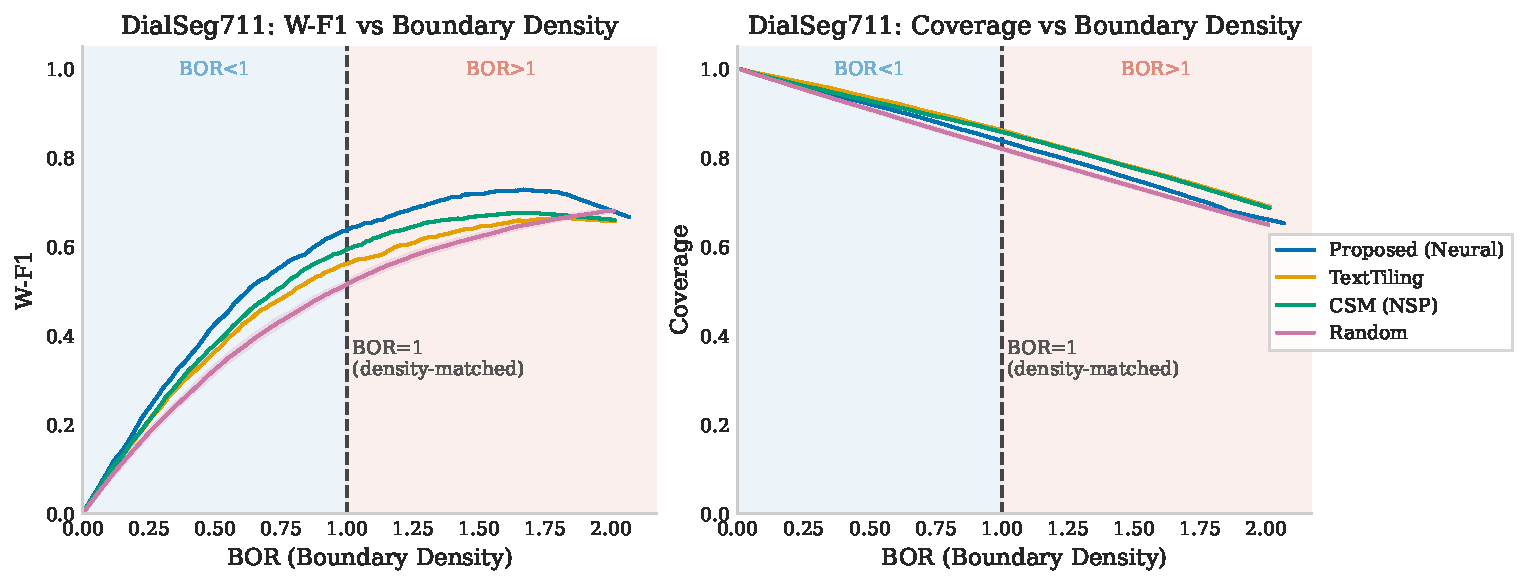
\includegraphics[width=\linewidth]{figures/density_quality_dialseg711_regimes.pdf}\\[2pt]
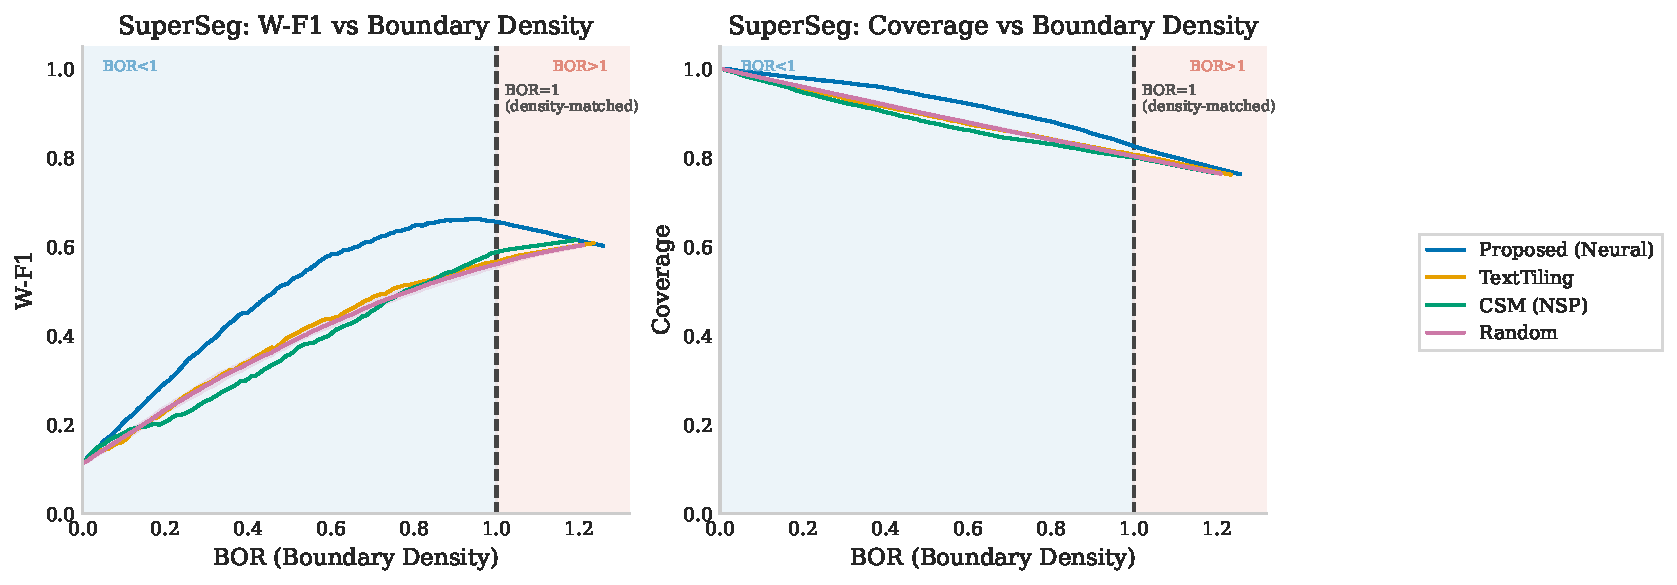
\includegraphics[width=\linewidth]{figures/density_quality_superseg_regimes.pdf}
\caption{\textbf{Density--quality curves for DialSeg711 and SuperSeg.}
Each curve varies the boundary-selection threshold for a fixed scoring model.
Horizontal movement (changing BOR) produces substantially larger changes in W-F1 and Coverage than vertical separation between methods, even for the proposed neural scorer.
SuperSeg exhibits a comparatively narrow optimum near BOR~$\approx 1$, while DialSeg711 tolerates a broader range of boundary densities, indicating dataset-dependent coupling between boundary-based metrics and annotation granularity.}
\label{fig:density-quality}
\end{figure}

\paragraph{Dataset-dependent density sensitivity.}
Figure~\ref{fig:density-quality} highlights a sharp contrast between SuperSeg and DialSeg711.
On SuperSeg, W-F1 is maximized near BOR~$\approx 1$ and degrades rapidly under under- or over-segmentation, indicating that evaluation strongly enforces the annotation boundary density.
On DialSeg711, by contrast, W-F1 exhibits a broad plateau across BOR, and oversegmentation is comparatively weakly penalized.
This contrast implies that identical boundary-based metrics can encode substantially different effective granularity assumptions across datasets.

Across both datasets, the proposed neural scorer is consistently higher than baselines at matched BOR, particularly in the conservative regime (BOR~$<1$), indicating improved boundary ranking; however, \emph{contrary to the standard assumption that boundary-based metrics primarily reward boundary placement once boundary density is fixed}, the dominant variation in W-F1 and Coverage is driven by boundary density shifts along each curve rather than by large vertical separation between methods.

\subsection{External Methods Under Granularity-Aware Evaluation}
To assess whether the granularity effects identified in this work are specific
to our scoring model or reflect broader evaluation behavior, we re-evaluated a
representative subset of published dialogue segmentation methods under the
proposed granularity-aware framework. The selected methods include simple
baselines (random and periodic segmentation), a classical unsupervised approach
(TextTiling), and a coherence-based model (CSM). All methods were evaluated using
the same boundary canonicalization and metrics as in previous sections.

\begin{table}[t]
\centering
\begin{tabular}{l l c c c c c}
\toprule
Method & Dataset & W-F1 & \textbf{BOR} & F1 & Purity & Coverage \\
\midrule
TextTiling & DialSeg711 & 0.648 & \textbf{1.88} & 0.550 & 0.968 & 0.746 \\
CSM        & DialSeg711 & 0.412 & \textbf{0.64} & 0.373 & 0.749 & 0.921 \\
Random     & DialSeg711 & 0.267 & \textbf{0.55} & 0.098 & 0.711 & 0.890 \\
Even       & DialSeg711 & 0.483 & \textbf{1.00} & 0.211 & 0.806 & 0.809 \\
\midrule
TextTiling & TIAGE      & 0.612 & \textbf{2.04} & 0.445 & 0.949 & 0.693 \\
CSM        & TIAGE      & 0.615 & \textbf{3.97} & 0.346 & 0.976 & 0.454 \\
Random     & TIAGE      & 0.256 & \textbf{0.33} & 0.121 & 0.697 & 0.921 \\
Even       & TIAGE      & 0.620 & \textbf{1.00} & 0.300 & 0.832 & 0.838 \\
\bottomrule
\end{tabular}
\caption{\textbf{External dialogue segmentation methods re-evaluated under the proposed
granularity-aware framework.} Boundary density (BOR) varies substantially across
methods and datasets, producing distinct density regimes despite comparable
boundary accuracy scores.}
\label{tab:external_methods}
\end{table}

Several patterns in Table~\ref{tab:external_methods} align with the
failure modes summarized in Table~\ref{tab:failure-taxonomy}. Simple
periodic segmentation achieves competitive boundary accuracy when its
output density aligns with the gold annotation (BOR $\approx 1$),
despite lacking semantic grounding. Classical methods such as
TextTiling exhibit recall-dominated behavior with elevated BOR,
yielding high purity alongside aggressive oversegmentation. Notably,
the same method (CSM) occupies different density regimes across
datasets, indicating that apparent performance differences often
reflect density mismatch rather than improved boundary detection. For
example, the regime shift observed for CSM across datasets is
consistent with differences in annotation density rather than changes
in boundary detection quality.

For clarity, and following the failure taxonomy in Table~\ref{tab:failure-taxonomy},
we categorize the results in Table~\ref{tab:external_methods} as conservative
(BOR $< 1$), balanced (BOR $\approx 1$), or aggressive (BOR $\gg 1$), as summarized
in Table~\ref{tab:regime_summary}.

\begin{table}[t]
\centering
\begin{tabular}{l l l}
\toprule
Method & Dataset & Density Regime \\
\midrule
TextTiling & DialSeg711 & Aggressive (BOR $\gg 1$) \\
CSM        & DialSeg711 & Conservative (BOR $< 1$) \\
Random     & DialSeg711 & Conservative (BOR $< 1$) \\
Even       & DialSeg711 & Balanced (BOR $\approx 1$) \\
\midrule
TextTiling & TIAGE      & Aggressive (BOR $\gg 1$) \\
CSM        & TIAGE      & Aggressive (BOR $\gg 1$) \\
Random     & TIAGE      & Conservative (BOR $< 1$) \\
Even       & TIAGE      & Balanced (BOR $\approx 1$) \\
\bottomrule
\end{tabular}
\caption{Density regimes under the proposed failure taxonomy, derived from BOR thresholds.
Regime labels are derived directly from BOR thresholds.}
\label{tab:regime_summary}
\end{table}

\paragraph{Targeted audit of runnable SuperDialseg leaderboard comparisons.}

Although these comparisons originate from the SuperDialseg benchmark leaderboard,
the audited methods are evaluated on DialSeg711 and TIAGE, which are included as
datasets within its evaluation suite.

To further examine how reported boundary-metric improvements relate to
segmentation granularity, we performed a targeted audit of three
runnable comparisons drawn from the SuperDialseg leaderboard. Each
comparison contrasts methods that differ in reported F1/W-F1 while
sharing the same evaluation protocol. These three comparisons exhaust
the set of SuperDialseg leaderboard comparisons that can be reproduced
using publicly available implementations without retraining or
proprietary APIs. We therefore restrict this audit to published
methods with deterministic implementations. The InstructGPT baseline
reported in SuperDialseg uses \texttt{text-davinci-003}, which has
since been deprecated and is no longer available; we do not reproduce
this baseline.

% Pairwise claim deltas for SuperDialseg audit (relative granularity shifts)
\begin{table}[t]
\centering
\small
\begin{tabular}{cllcccc}
\toprule
Claim & Comparison & Dataset & $\Delta$F1 & $\Delta$W-F1 & $\Delta$BOR & Relative Density Shift \\
\midrule
A & TextTiling vs.\ CSM & DialSeg711 & +0.135 & +0.220 & +2.13 & Conservative $\rightarrow$ Aggressive \\
B & TextTiling vs.\ CSM & TIAGE & +0.128 & +0.219 & +1.26 & Aggressive $\rightarrow$ More Aggressive \\
C & TextTiling vs.\ Even & DialSeg711 & +0.277 & +0.132 & +1.69 & Balanced $\rightarrow$ Aggressive \\
\bottomrule
\end{tabular}
\caption{Pairwise audit of runnable SuperDialseg leaderboard comparisons. For each claim,
positive $\Delta$ indicates higher values for the first-listed method. Arrows denote
relative changes in boundary density from the second-listed method to the first-listed
method, not absolute regime membership. Regime labels follow the thresholds defined
in Table~\ref{tab:failure-taxonomy}.}
\label{tab:leaderboard-deltas}
\end{table}

\paragraph{Concrete example of a likely confounded comparison.}
Table~5 provides a direct illustration of how published boundary-metric ``improvements'' can be driven by
density regime shifts rather than improved boundary placement.
For example, on DialSeg711, the comparison \emph{TextTiling vs.\ CSM} shows a substantial increase in
W-F1 ($\Delta$W-F1 $= +0.220$) accompanied by a large increase in boundary density
($\Delta$BOR $= +2.13$), moving from a conservative regime (BOR $<1$) to an aggressive regime
(BOR $\gg 1$).
Under the failure taxonomy in Table~1, this pattern is consistent with recall-dominated oversegmentation:
higher tolerant boundary scores arise from emitting many more boundaries, not necessarily from more accurate
boundary localization at a matched granularity.
This is precisely the confound our reporting framework is designed to expose: W-F1 alone does not
distinguish a genuine detection improvement from a density-driven regime change.

This behavior aligns with the failure modes summarized in
Table~\ref{tab:failure-taxonomy}, where recall-dominated
oversegmentation yields higher boundary accuracy under tolerant
metrics despite substantial shifts in segmentation granularity.

\subsection{Stage 1: Synthetic Pretraining on Splice Boundaries}
This stage isolates whether the scoring model can learn a meaningful boundary
signal in a controlled setting, independent of annotation noise.
Performance here reflects the model's ability to distinguish genuine topic
transitions from non-boundaries before exposure to real dialogue benchmarks.
Table~\ref{tab:stage1} summarizes boundary-level behavior during this phase.

\begin{table}[t]
\centering
\begin{tabular}{ccccccl}
\toprule
Epoch & F1 & W-F1 & BOR & Mean $|$score$|$ & Neg.\ Ctrl.\\
\midrule
1 & 0.265 & 0.420 & 0.31 & 0.007 & 0.000 \\
2 & 0.453 & 0.688 & 0.67 & 0.009 & 0.032 \\
3 & 0.489 & 0.733 & 0.87 & 0.010 & —  \\
\bottomrule
\end{tabular}
\caption{\textbf{Stage 1 synthetic pretraining on splice boundaries.}
Mean $|$score$|$ denotes the mean boundary score magnitude $\mathbb{E}[|s_i|]$ on the validation set and serves as a diagnostic for score collapse. Negative control (Neg.\ Ctrl.) reports the predicted boundary rate on single-segment dialogues,
which should be near zero; it was not rerun for epoch 3, as the model had already passed this sanity check at epoch 2.
}
\label{tab:stage1}
\end{table}

\subsection{Stage 2: Supervised Fine-Tuning on Benchmarks}
This stage evaluates how supervised fine-tuning aligns the scoring model with
human annotation conventions on in-distribution datasets.
The key question is whether boundary density stabilizes without degrading
boundary ranking quality.
Table~\ref{tab:stage2} reports performance over five fine-tuning epochs.

\begin{table}[t]
\centering
\begin{tabular}{c c c c c c}
\toprule
Epoch & Overall F1 & W-F1 & \textbf{BOR} & SuperSeg F1/BOR & TIAGE F1/BOR \\
\midrule
1 & 0.778 & 0.833 & \textbf{1.11} & 0.788 / 1.13 & 0.197 / 0.24 \\
2 & 0.819 & 0.850 & \textbf{1.23} & 0.830 / 1.25 & 0.352 / 0.86 \\
3 & 0.840 & 0.865 & \textbf{1.13} & 0.852 / 1.14 & 0.337 / 0.82 \\
4 & 0.848 & 0.875 & \textbf{1.08} & 0.862 / 1.08 & 0.322 / 0.78 \\
5 & 0.843 & 0.872 & \textbf{1.04} & 0.857 / 1.05 & 0.311 / 0.84 \\
\bottomrule
\end{tabular}
\caption{\textbf{Stage 2 supervised fine-tuning on benchmark datasets.}
Boundary density converges toward annotated density (BOR $\approx 1$) on datasets seen during training,
while W-F1 remains high.}
\label{tab:stage2}
\end{table}

\subsection{Stage 3: Final Test with Calibration}
\label{sec:stage3}
This stage evaluates generalization under distribution shift, where annotation
granularity differs from the training regime.
Here, the focus is not peak F1 but the interaction between boundary ranking,
boundary density, and calibration.

Final test results are shown in Table~\ref{tab:stage3}, which reports
evaluation metrics for a representative subset of three datasets
spanning sparse, medium, and dense annotation regimes; results on the
remaining datasets follow the same qualitative pattern.

\begin{table}[t]
\centering
\begin{tabular}{lcccc}
\toprule
Dataset & W-F1 & \textbf{BOR} & F1 & Pred./Gold Boundaries \\
\midrule
DialSeg711 & 0.767 & \textbf{2.53} & 0.434 & 5167/2042 \\
SuperSeg   & 0.584 & \textbf{0.81} & 0.609 & 2376/2923 \\
TIAGE      & 0.512 & \textbf{0.76} & 0.368 & 157/207 \\
\bottomrule
\end{tabular}
\caption{\textbf{Stage 3 final test results.}
Boundary density (BOR) is reported alongside boundary accuracy to distinguish
granularity mismatch from detection failure.}
\label{tab:stage3}
\end{table}

\noindent\textbf{Calibration.}
We learned a single global temperature of $T = 0.976$ for this run.
In practice, temperature scaling modestly improves score calibration and
threshold stability, but it does not eliminate cross-dataset threshold
non-transfer: differences in annotation granularity continue to dominate the
relationship between score thresholds and boundary density.

Complete Stage~3 calibrated results for all eight datasets are reported in Appendix~\ref{app:stage3}.

\section{Segment Coherence Diagnostics}

These coherence diagnostics are essential for interpreting boundary-based
metrics under granularity mismatch. In particular, they distinguish between
two qualitatively different outcomes that exact-match metrics conflate:
(1) segmentations that introduce additional but coherent subtopic boundaries,
and (2) segmentations that fragment topics into incoherent or mixed segments.

As shown in Table~\ref{tab:purity_coverage}, the proposed model
maintains high purity across datasets even when boundary density
exceeds that of the gold annotation. When considered conditional on
non-trivial boundary detection performance (W-F1) and relative to the
random (BOR=1) baseline, this pattern is \emph{consistent with} the
additional predicted boundaries aligning with meaningful conversational
structure rather than being purely density-driven artifacts. In contrast,
baseline methods with matched boundary density achieve competitive
boundary metrics but exhibit lower or unstable coherence, underscoring
that density alignment alone does not guarantee usable segmentation.

Taken together, these results demonstrate that segment coherence metrics are
necessary to interpret boundary accuracy meaningfully when annotation
granularity varies, and that high BOR should not be interpreted as failure
in the presence of high purity and coverage.

\begin{table}[t]
\centering
\begin{tabular}{l c c c c c}
\toprule
Dataset & W-F1 & \textbf{BOR} & Purity & Coverage & F1 \\
\midrule
 DialSeg711 & 0.767 & \textbf{2.53} & 0.962 & 0.651 & 0.434 \\
 SuperSeg   & 0.584 & \textbf{0.81} & 0.847 & 0.915 & 0.609 \\
 TIAGE      & 0.512 & \textbf{0.76} & 0.785 & 0.896 & 0.368 \\
\bottomrule
\end{tabular}
\caption{\textbf{Segment coherence diagnostics for the proposed model.}
High purity with elevated BOR indicates coherent fine-grained segmentation; high
coverage with reduced BOR indicates coarser-than-gold segmentation. Both patterns
reflect granularity mismatch rather than boundary detection failure.}
\label{tab:purity_coverage}
\end{table}

\subsection{Worked Example}
We illustrate the effect of annotation granularity on evaluation metrics using
a short dialogue example with both coarse gold boundaries and fine-grained model
predictions in Figure~\ref{fig:worked_example}.

This example makes concrete the failure mode identified throughout the paper.
The predicted boundaries correspond to coherent conversational subtopics that
are omitted by the coarse gold annotation. Under exact-match evaluation, these
additional boundaries are treated as false positives, substantially reducing
F1 despite correct identification of the major topic transition. The example
therefore highlights that the dominant error is one of boundary density rather
than boundary placement, and motivates evaluation criteria that distinguish
granularity mismatch from detection failure.

\begin{figure}[t]
\centering
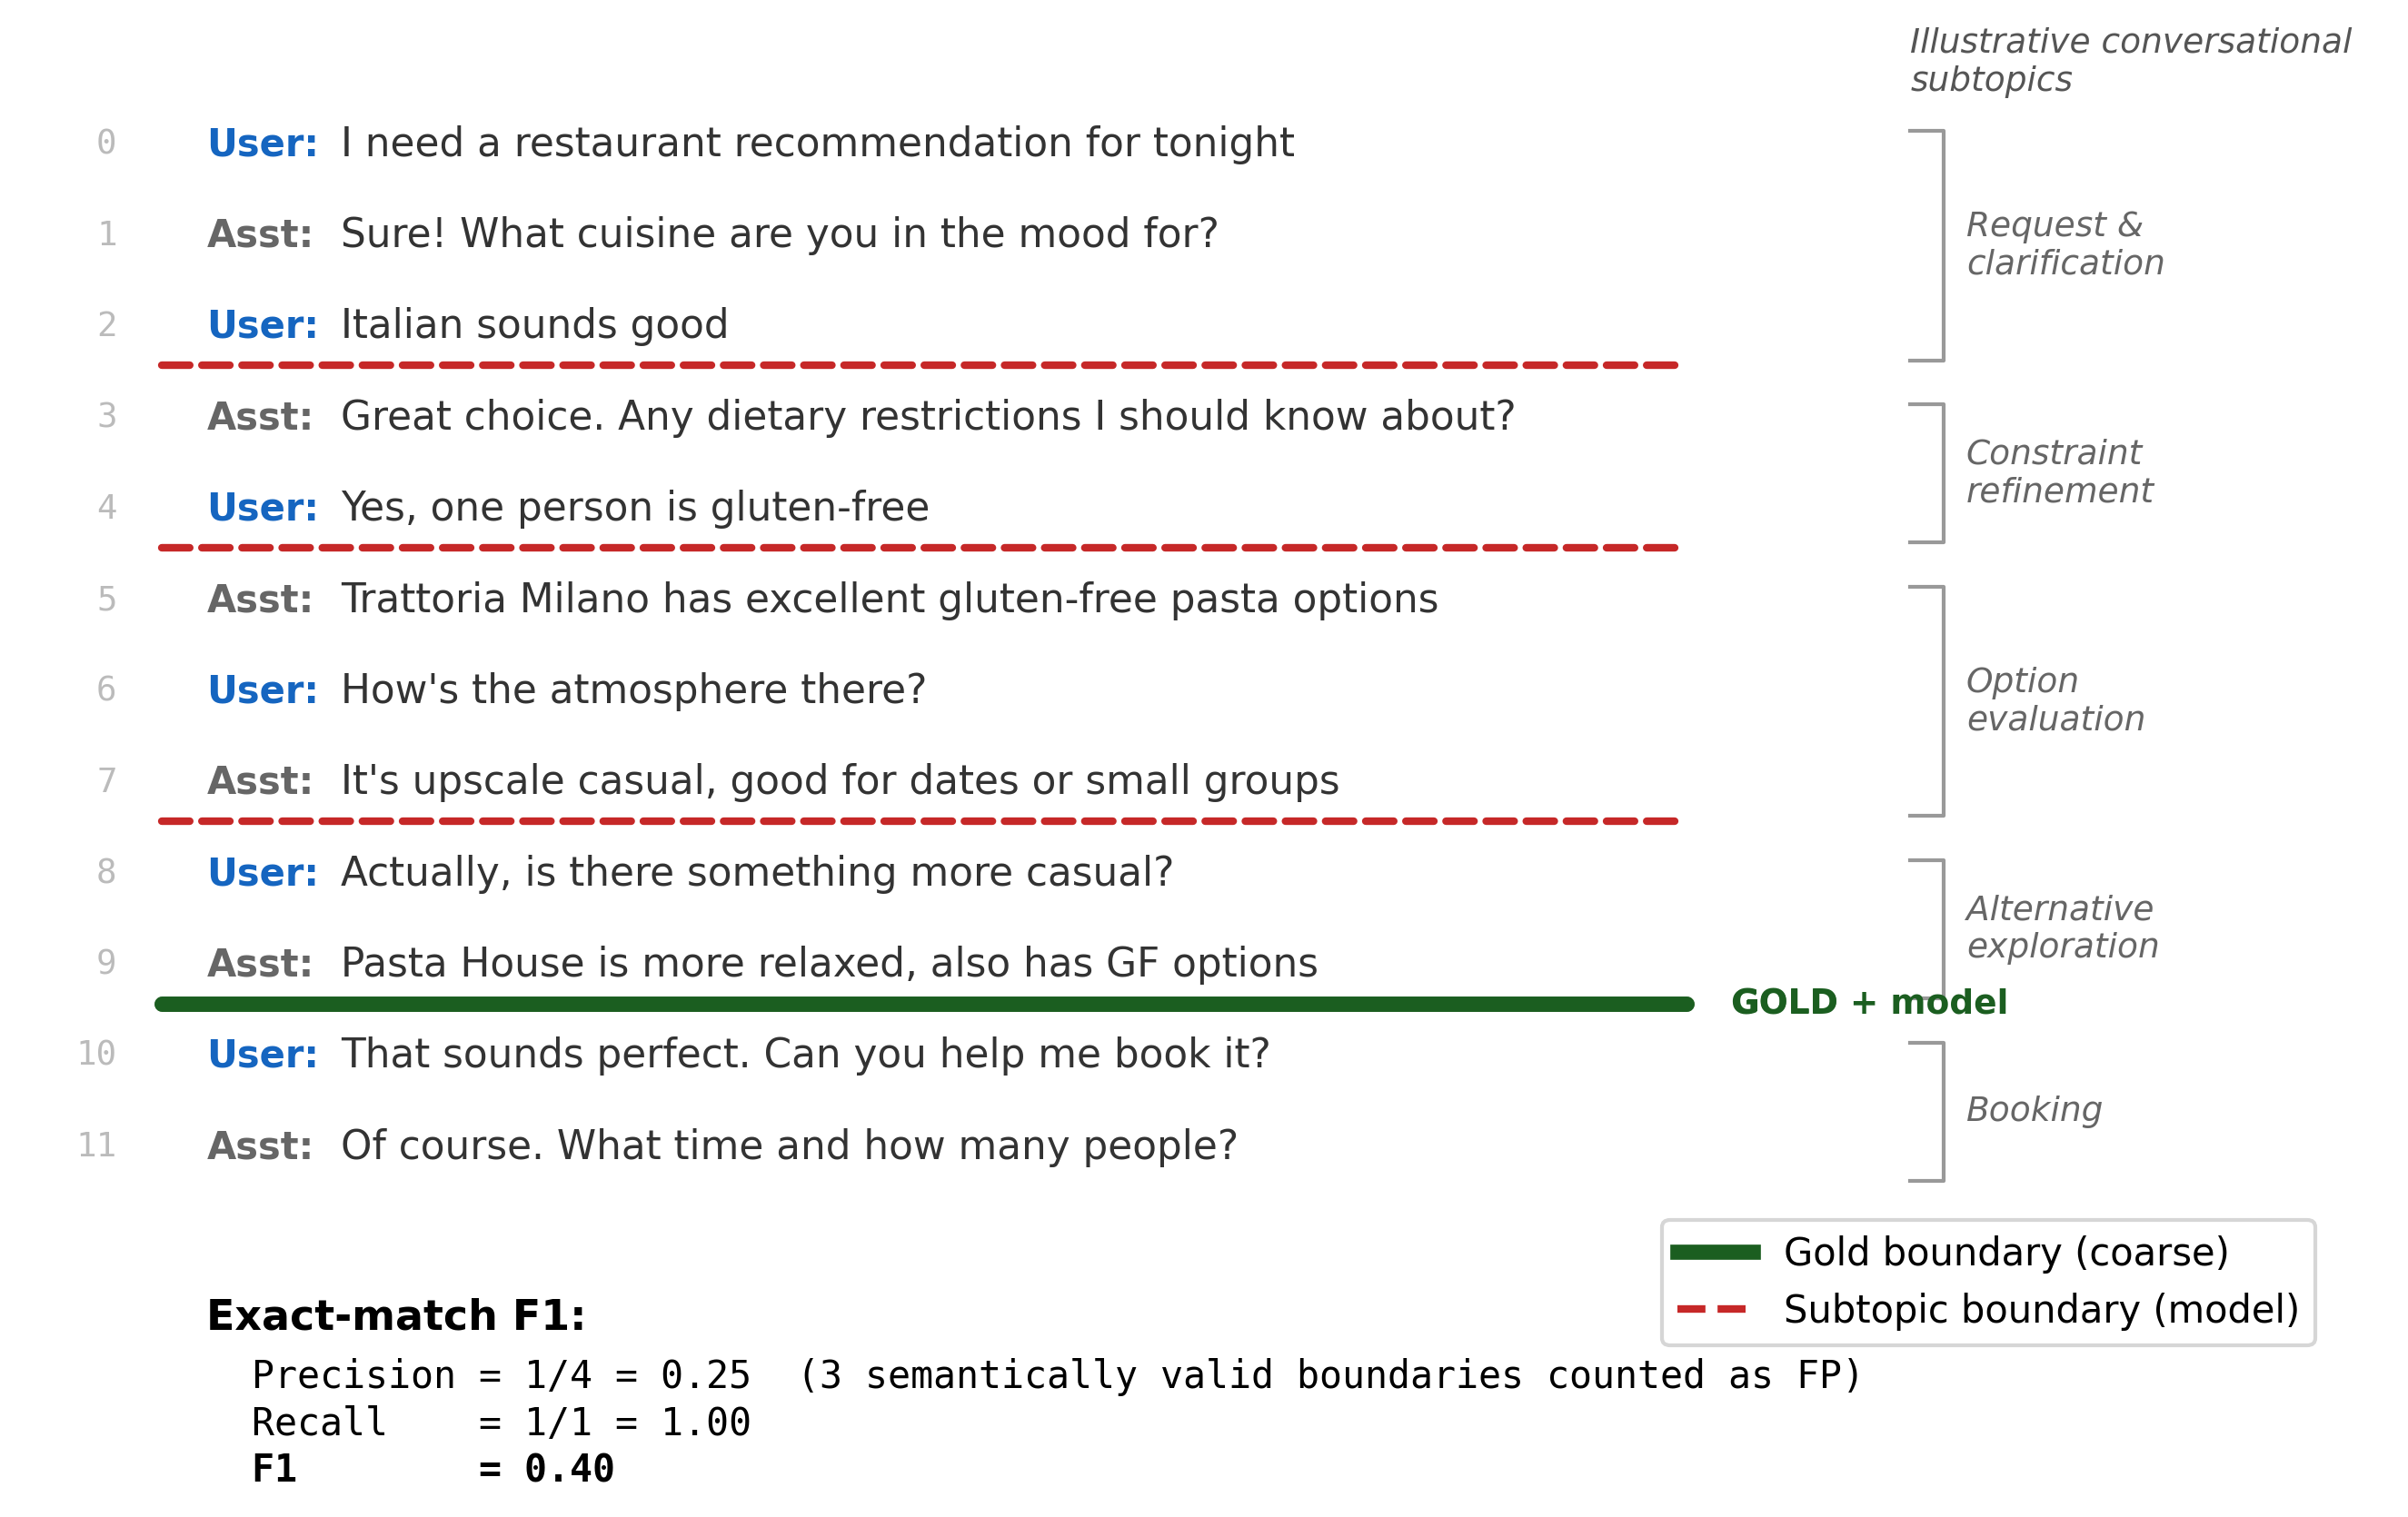
\includegraphics[width=\linewidth]{figures/granularity_mismatch.png}
\caption{
\textbf{Granularity mismatch in dialogue topic segmentation.}
Gold annotations mark a single coarse topic boundary (browsing $\rightarrow$ booking),
while the model identifies multiple semantically meaningful subtopic transitions.
The fine-grained boundaries correspond to coherent conversational phases and are
not boundary-positioning errors. Under exact-match evaluation, three valid predicted subtopic boundaries are counted as false positives, yielding F1=0.40 despite correct
identification of the coarse transition. The error arises from a mismatch in
boundary density and segmentation granularity rather than from incorrect
boundary detection.}
\label{fig:worked_example}
\end{figure}

\section{Discussion}
The results demonstrate that boundary-based accuracy metrics conflate
segmentation quality with boundary density alignment when annotation
granularity varies. In particular, the apparent competitiveness of
oracle-density baselines in Table~\ref{tab:baselines} should not be
interpreted as modeling capability, but as evidence that boundary
accuracy metrics reward density alignment rather than transferable
boundary detection.  Baseline comparisons in Table~\ref{tab:baselines}
expose a central weakness of standard boundary-based metrics: random
and periodic strategies achieve competitive W-F1 and purity scores
when their output boundary density is matched to the gold annotation,
despite lacking any semantic grounding. In contrast, the proposed
model yields substantially higher segment purity on datasets with
coarse annotations, at the cost of elevated BOR, indicating coherent
fine-grained segmentation rather than detection failure.

Figure~\ref{fig:density-quality} reinforces this point by showing that
the variation in W-F1 induced by sweeping the boundary selection threshold
for a fixed scoring model (moving along a curve) is substantially larger
than the variation observed between segmentation methods at a matched
boundary density.
\emph{This behavior is contrary to the standard evaluation assumption
that boundary-based metrics primarily reflect boundary placement quality
once density is controlled.}
We intentionally do not prescribe a universal target BOR, as any such
prescription would reintroduce a single ``correct'' granularity that this
work argues does not exist.

Importantly, this evaluation failure is not model-specific: any method
whose output boundary density is tuned to match the gold annotation
can achieve competitive F1 and W-F1 scores, as demonstrated by the
non-semantic baselines in Table~\ref{tab:baselines}. We do not attempt
a comprehensive retrospective survey of published claims across all
leaderboards and datasets; instead, we provide targeted, runnable
audits (Table~5) that concretely demonstrate how apparent
boundary-metric gains can arise from substantial shifts in boundary
density regimes. Adding more segmentation models does not resolve this
problem; it only illustrates it further.

Additional experiments with classical change-detection and drift-based
strategies further support this conclusion. Such methods (e.g., cumulative-sum
and time-aware change detection) often achieve higher W-F1 than the neural
scorer by aggressively increasing boundary density, frequently yielding
boundary oversegmentation ratios well above~1.0. This demonstrates that strong
boundary accuracy under tolerant metrics can be driven by recall-dominated
strategies rather than by calibrated segmentation aligned with downstream use.
The proposed evaluation objective makes this trade-off explicit: methods with
higher W-F1 but elevated BOR are correctly identified as oversegmenting, while
more conservative scorers exhibit lower boundary accuracy but better density
control.

Across the methods examined in this study, three qualitatively distinct
density regimes emerge:
\begin{itemize}
\item \textbf{Conservative strategies} (e.g., SpeechAct, SummaryProbe)
undersegment, producing $\text{BOR} < 1$ and low recall.
\item \textbf{Balanced strategies} (e.g., Neural(fine), density-matched
selection) achieve $\text{BOR} \approx 1$ with high segment purity, yielding
calibrated segmentation aligned with annotation density.
\item \textbf{Aggressive strategies} (e.g., CUSUM, time-aware drift detection)
maximize recall and W-F1 by substantially increasing boundary density
($\text{BOR} \gg 1$), resulting in recall-dominated detection rather than
calibrated segmentation.
\end{itemize}

To confirm that granularity effects are not specific to our scorer, we
evaluated CSM~\cite{xing2021csm}, a published coherence-based
segmentation model, under the same framework. CSM operates in the
conservative regime (BOR=0.64), producing fewer boundaries than the
gold annotation. Its low strict F1 (0.373) reflects low recall rather
than incoherent segmentation: coverage remains high (0.921),
indicating that predicted segments are valid but coarser than the
reference. This demonstrates that the granularity-F1 interaction
identified here generalizes across structurally distinct segmentation
methods.

In practice, selection thresholds should therefore be chosen based on intended
downstream use rather than optimized solely to match a particular annotation
density. Boundary density metrics such as BOR provide a simple diagnostic for
tuning selection behavior without retraining the scoring model.

\paragraph{Practical guidance for choosing boundary density.}
The appropriate boundary selection behavior depends on how segmentation outputs
are used downstream. Based on the empirical results in this study, we offer the
following high-level guidance:

\begin{itemize}
\item \textbf{Summarization and context truncation.}
When topic boundaries trigger summarization or removal of prior turns, missing a
major boundary can be more harmful than introducing extra minor boundaries.
Conservative selection is therefore preferable: a lower boundary density
($\text{BOR} < 1$) reduces the risk of prematurely discarding relevant context,
even if some distinct topics are merged.

\item \textbf{Retrieval and navigation.}
For applications that rely on topic boundaries to index or retrieve relevant
conversation segments, finer-grained segmentation can be beneficial provided
segments remain coherent. In this regime, higher boundary density
($\text{BOR} > 1$) is acceptable as long as purity remains high, indicating that
additional boundaries correspond to meaningful subtopics rather than noise.

\item \textbf{Exploratory analysis and annotation.}
When segmentation is used for qualitative analysis, annotation support, or
exploratory inspection, fine-grained boundaries are often desirable. In such
settings, boundary density may substantially exceed that of existing
annotations, and evaluation should emphasize segment coherence over exact
boundary alignment.
\end{itemize}

These guidelines reinforce the central claim of this paper: boundary density is
not an intrinsic property of a conversation, but a design choice that should be
tuned to application requirements rather than optimized to match a given
annotation scheme. This dependence on selection behavior motivates treating
boundary selection as a distinct, explicit step.

\subsection{Boundary Selection as a Separate Step}
\label{sec:boundary-selection}
Separating boundary scoring from boundary selection makes boundary density an explicit control
parameter rather than an incidental consequence of threshold tuning.

Figure~\ref{fig:adaptive_commitment} illustrates the consequence of
this separation: different scoring granularities produce substantially
different candidate boundary rates, yet an explicit selection rule
enforces stable output boundary distributions that are invariant to
the scorer's granularity. Crucially, this invariance does not arise
from score rescaling or post-hoc normalization.  The scoring function
is unchanged; identical output distributions emerge solely from the
selection mechanism's evidence accumulation and adaptive thresholding
behavior.  This behavior illustrates that separating scoring from
selection enables boundary density to be controlled independently of
scoring granularity, motivating its treatment as a design parameter
rather than an evaluation artifact. A fully specified and
reimplementable version of this adaptive controller is given in
Appendix~\ref{app:adaptive}.


\begin{figure*}[t]
\centering
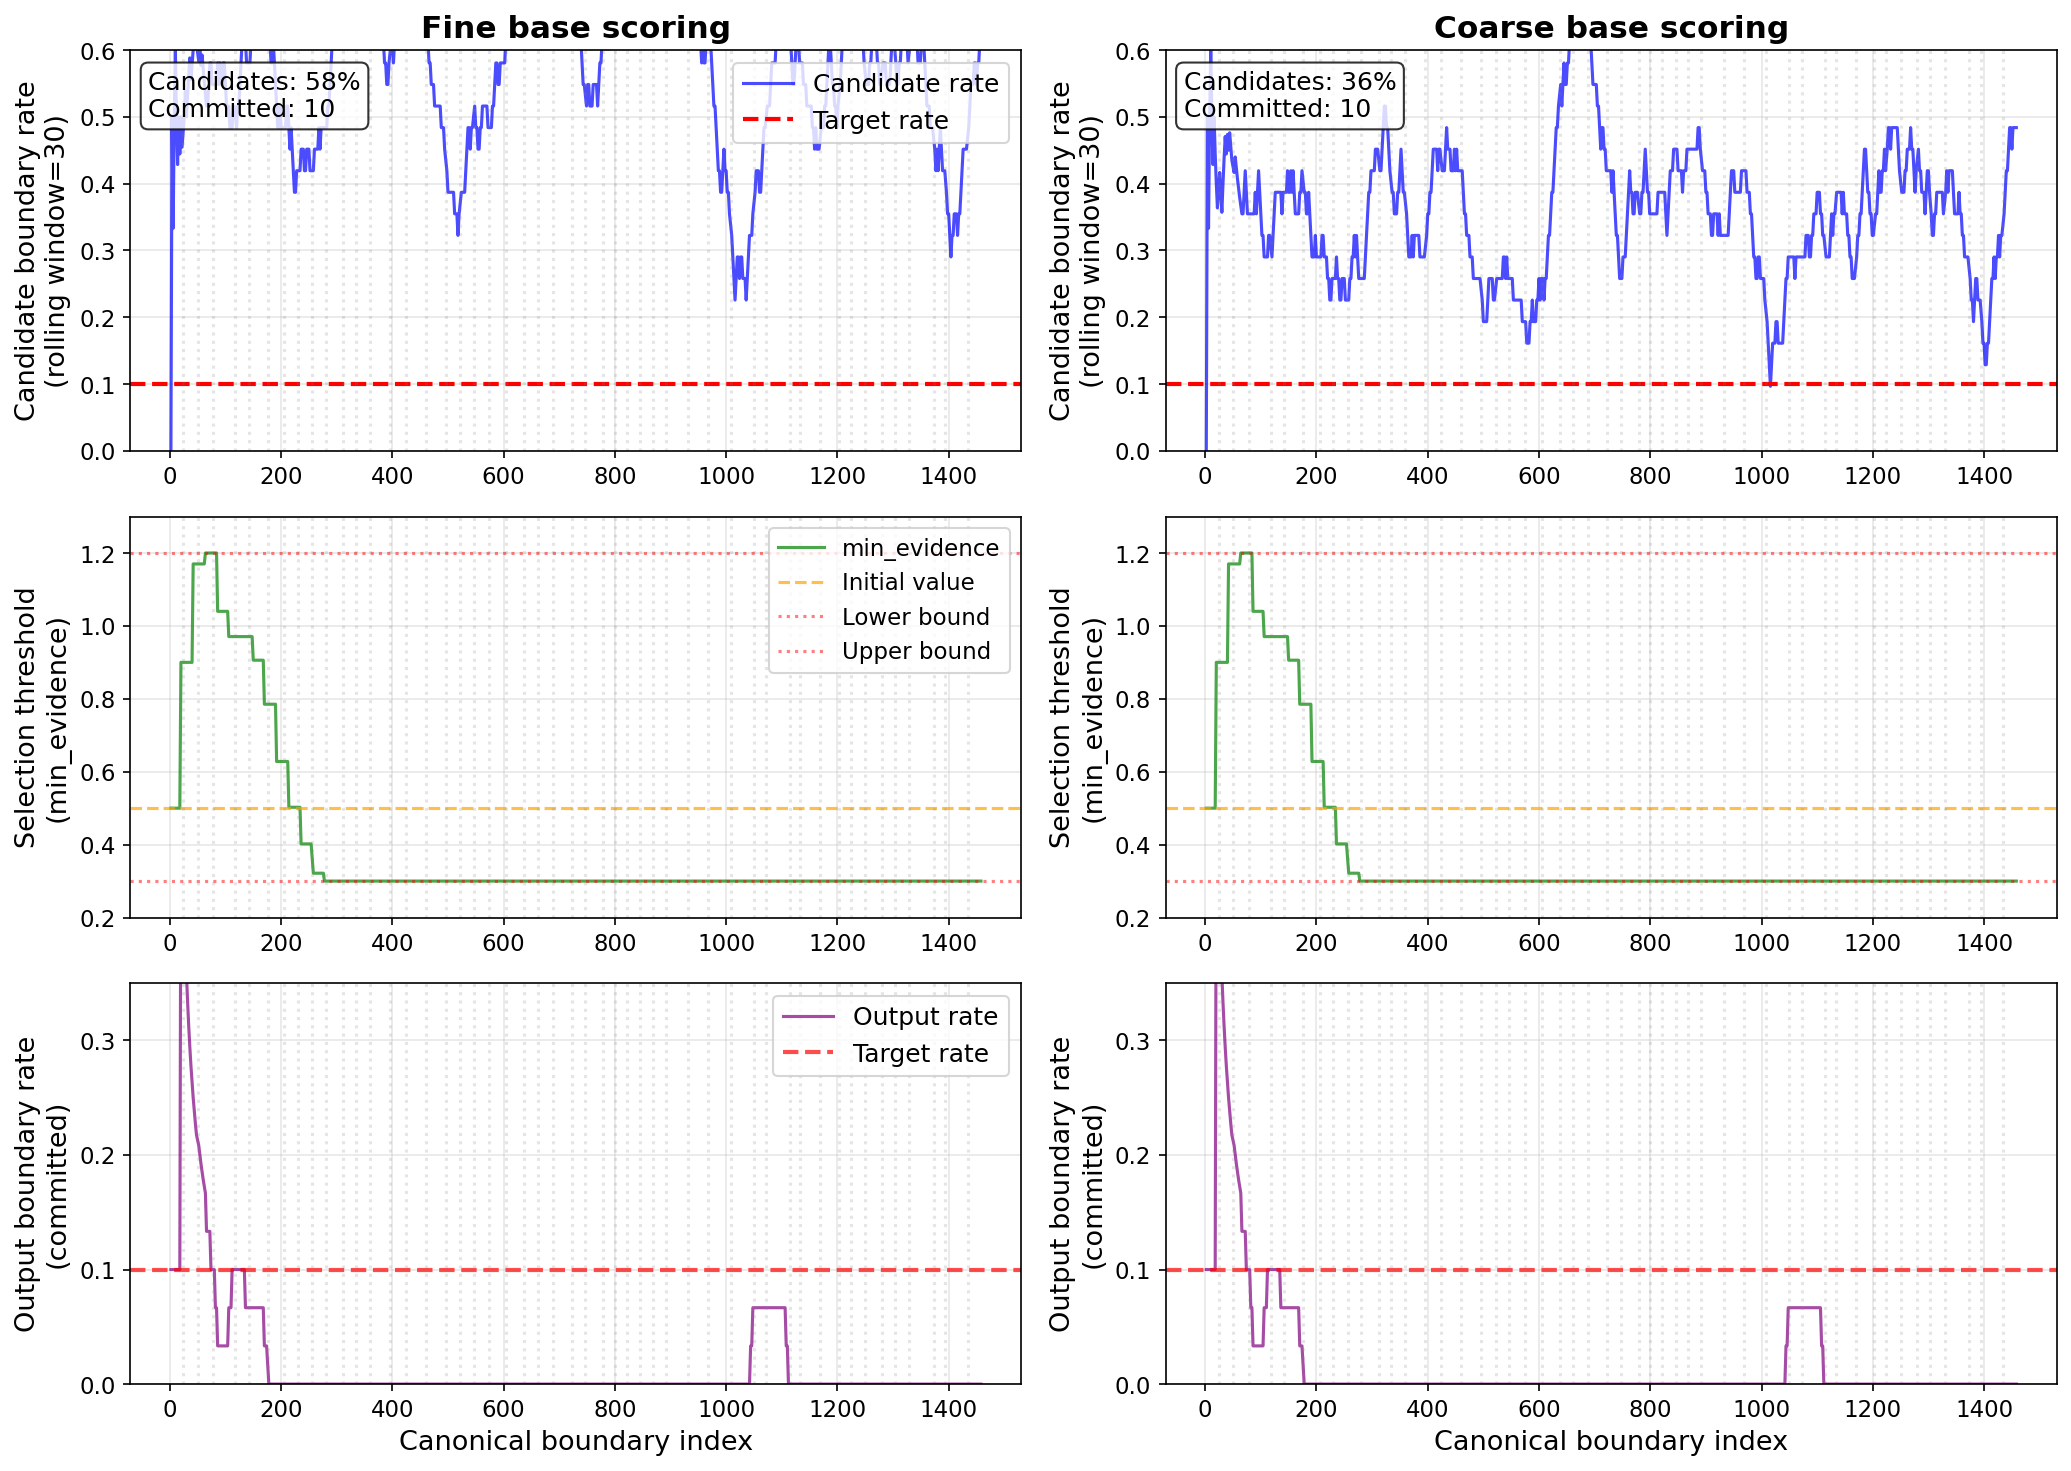
\includegraphics[width=\textwidth]{figures/adaptive_commitment_granularity.png}
\caption{\textbf{Adaptive boundary selection enforces invariant boundary distributions across scoring granularities (DialSeg711).}
\emph{Top row} shows the raw candidate boundary rate produced by the same scorer under fine
(left) and coarse (right) candidate thresholds, resulting in substantially different candidate
frequencies (73.5\% vs.\ 57.7\%). The dashed line indicates the target selection rate specified to the
controller. \emph{Bottom row} shows the resulting distribution of selected boundaries over message
index after adaptive thresholding. Despite large differences in candidate generation, adaptive
selection converges to nearly identical boundary distributions and total selection counts
(16.7\% selection rate, $N{=}542$ in both cases). This invariance is \emph{not} the result of score
rescaling or post-hoc normalization: the underlying scoring function is unchanged, and the effect
emerges from online evidence accumulation and adaptive thresholding, reflecting successful decoupling of
boundary selection from boundary scoring. The adaptive selection procedure illustrated here is formally specified in
Appendix~\ref{app:adaptive}.}
\label{fig:adaptive_commitment}
\end{figure*}

\subsection{Computational Cost}

Boundary selection is computationally negligible: it operates on a vector of scores and applies thresholding and minimum spacing. Boundary scoring dominates cost because it requires running the neural model over candidate positions (window-vs-window inputs around each position). The separation therefore has practical value in deployed systems: selection can be retuned per dataset or application without recomputing scores, while recomputing scores requires model inference. Evidence accumulation within online boundary selection is likewise lightweight relative to scoring, since it reuses the fixed-reference scores and maintains only decision state.

\subsection{On Dataset Choice and External Validity}

Public dialogue datasets are necessarily imperfect proxies for real human–AI
interactions. While several conversational AI datasets have been released, we
are not aware of any publicly available corpus of long, open-ended human–AI
conversations with turn-level topic boundary annotations suitable for evaluating
segmentation granularity. Our claims therefore concern evaluation behavior under
heterogeneous annotation schemes rather than direct modeling of user behavior.
The consistency of failure modes across diverse datasets indicates that these
effects arise from evaluation practice rather than dataset-specific artifacts.

\section{Limitations and Future Work}

This work does not introduce a new neural backbone for dialogue topic
segmentation.
Instead, it contributes (i) an evaluation objective that makes boundary density
and segment coherence explicit and (ii) a topic segmentation algorithm that
separates boundary scoring from boundary selection.
We do not include a direct ablation comparing synthetic pretraining against
training from scratch. 
Preliminary experiments indicate that splice-boundary pretraining primarily
stabilizes early training dynamics rather than improving final performance, but
a systematic ablation remains an important direction for future work. 

Purity and coverage are computed with respect to the same gold annotations whose
granularity we argue is often mismatched to model behavior.
Accordingly, these measures should not be interpreted as independent estimates
of semantic coherence.
Rather, they function as relative diagnostics: high purity rules out incoherent
mixing of gold topics, while elevated BOR distinguishes fine-grained subdivision
from boundary noise.
Independent coherence measures (e.g., embedding-based similarity or human
judgments) would be valuable complements, but are not required for the present
goal of diagnosing evaluation failure modes under mismatched annotation
granularity.

\paragraph{Interpretation constraint.}
Purity and coverage should only be interpreted conditional on
non-trivial boundary detection performance (e.g., W-F1 significantly
greater than zero). When considered in isolation, both measures can be
arbitrarily high or low for segmentations with no semantic content,
including density-matched random baselines.

\paragraph{Statistical variability.}
We do not report confidence intervals or significance tests for the metrics
presented in this work.
Our primary claims concern qualitative failure modes and regime-level behavior
(e.g., recall-dominated oversegmentation versus calibrated segmentation), which
manifest as large and consistent differences in boundary density and coherence
across datasets and methods.
In preliminary experiments, variance across random seeds and training runs was
small relative to these effects and did not alter the qualitative conclusions.
Future work could include multi-run statistical reporting for finer-grained
comparisons within a given density regime, but such analysis is not
required to support the central evaluation claims made here.

Inter-annotator agreement (IAA) statistics could also provide additional
empirical support for the claim that topic boundaries are granularity-dependent
rather than objective.
Several dialogue segmentation datasets report IAA in their original
publications (e.g., DialSeg711~\cite{dialseg711}, SuperDialseg~\cite{superdialseg2023}), often showing only moderate agreement even under controlled
annotation protocols.
However, these statistics are reported using heterogeneous definitions and
units (e.g., boundary placement, segment overlap, or task-level agreement),
making direct comparison across datasets difficult.
Because the present work focuses on evaluation behavior under fixed annotation
schemes rather than on the reliability of those schemes themselves, we do not
reanalyze annotator agreement here.
Integrating IAA into a unified analysis of granularity effects remains an
important direction for future work.

Additional directions include evaluating published dialogue segmentation methods
under the proposed evaluation objective to confirm that the observed granularity
effects are method-agnostic, and exploring alternative boundary selection rules
that adapt boundary density to application constraints rather than annotation
conventions.
Further study is also needed to relate boundary density preferences to specific
downstream uses such as summarization, retrieval, or conversational memory.
Finally, future work could replace discrete boundary representations with
continuous or multi-scale topic representations (e.g., topic clouds) that better
capture overlapping, gradual, or revisited conversational structure.

\section{Conclusion}

Dialogue topic segmentation does not admit a single ground
truth. Exact boundary matching conflates detection correctness with
segmentation granularity and can obscure coherent segmentation
behavior under differing annotation granularity.  By evaluating
boundary density and segment coherence alongside W-F1, this work
provides a principled basis for diagnosing evaluation failures across
datasets.

A central empirical finding is that boundary-based metrics can be
dominated by boundary density alignment. For example, we observe that
the same published method (CSM) occupies different density regimes
across datasets, a pattern consistent with differences in annotation
density rather than changes in boundary detection quality. This
underscores that boundary accuracy alone is insufficient when
annotation granularity varies. For example, a targeted audit of
runnable SuperDialseg method comparisons shows that higher boundary
accuracy is consistently accompanied by shifts toward more aggressive
density regimes, rather than by improved boundary placement.

The proposed separation is intentionally simple. Its value lies in
revealing systematic evaluation failures that arise when granularity
is ignored. Our goal is not to claim model superiority, but to
motivate reporting practices that make boundary density and segment
coherence explicit. We expect these diagnostics to be useful both for benchmarking research
systems and for analyzing and configuring segmentation choices in practice.

\FloatBarrier
\appendix
\section{W-F1 definition (matching, empty-set policy, aggregation)}
\label{app:wf1}

Let $w$ be the tolerance window (we use $w=1$, i.e., a $\pm 1$ message tolerance window).
For each dialogue $d$ with gold boundaries $G_d \subset \{1,\dots,T_d-1\}$ and predicted
boundaries $P_d \subset \{1,\dots,T_d-1\}$, define:
\[
\mathrm{TP}_d = \left|\left\{p \in P_d : \exists\, g \in G_d \text{ s.t. } |p-g|\le w\right\}\right|,\quad
\mathrm{MG}_d = \left|\left\{g \in G_d : \exists\, p \in P_d \text{ s.t. } |p-g|\le w\right\}\right|.
\]
That is, a predicted boundary is counted as correct if it lies within $\pm w$ of any
gold boundary, and a gold boundary is counted as recovered if any prediction lies within
$\pm w$ of it. Under this window-coverage convention, a single gold boundary may satisfy
multiple predictions, while each gold boundary contributes at most once to recall.

Precision and recall are computed per dialogue with explicit empty-set handling:
\[
\mathrm{Prec}_d =
\begin{cases}
\mathrm{TP}_d/|P_d| & |P_d|>0\\
1 & |P_d|=0 \land |G_d|=0\\
0 & |P_d|=0 \land |G_d|>0
\end{cases}
\qquad
\mathrm{Rec}_d =
\begin{cases}
\mathrm{MG}_d/|G_d| & |G_d|>0\\
1 & |G_d|=0 \land |P_d|=0\\
0 & |G_d|=0 \land |P_d|>0
\end{cases}
\]
\[
\mathrm{W\text{-}F1}_d =
\begin{cases}
\frac{2\,\mathrm{Prec}_d\,\mathrm{Rec}_d}{\mathrm{Prec}_d+\mathrm{Rec}_d} & \mathrm{Prec}_d+\mathrm{Rec}_d>0\\
0 & \text{otherwise.}
\end{cases}
\]

We report \emph{dialogue-level macro} W-F1, i.e.,
$\mathrm{W\text{-}F1}=\frac{1}{|D|}\sum_{d\in D}\mathrm{W\text{-}F1}_d$.
This aggregation implies that the no-boundary baseline can attain nonzero macro W-F1 on datasets
that include dialogues with no gold boundaries. In particular, if both gold and predicted boundary
sets are empty for a dialogue, then $\mathrm{Prec}_d=\mathrm{Rec}_d=1$ and $\mathrm{W\text{-}F1}_d=1$ under the
convention above.

\section{Full Stage~3 Calibrated Results Across All Datasets}
\label{app:stage3}

The main text (Section~\ref{sec:stage3}) reports Stage~3 calibrated results on three
representative datasets spanning sparse, medium, and dense annotation
regimes. To substantiate the cross-dataset claims made in Sections~4 and~7,
this appendix reports the same Stage~3 evaluation
metrics for all eight datasets used in this study: DialSeg711,
SuperDialseg (SuperSeg), TIAGE, MultiWOZ, DailyDialog, Taskmaster,
Topical-Chat, and QMSum.

All results in Table~\ref{tab:stage3-all8} were computed using the
identical Stage~3 evaluation pipeline as the main Stage~3 results
(Table~\ref{tab:stage3}): a single globally calibrated temperature
($T=0.976$), identical boundary canonicalization, fixed boundary
selection parameters, and the evaluation definitions in Section~\ref{sec:evaluation-metrics}.

We report window-tolerant boundary detection (W-F1 with a $\pm 1$
message tolerance), boundary density relative to gold annotations
(BOR), and segment coherence diagnostics (purity and coverage), along
with predicted and gold boundary counts. Strict exact-match boundary
F1 is omitted here because it is highly sensitive to aggregation
choice (e.g., micro vs.\ macro averaging) and boundary sparsity, and
it is not a primary diagnostic in the proposed evaluation objective.

\begin{table*}[t]
\centering
\small
\begin{tabular}{lcccccc}
\toprule
Dataset & W-F1 & BOR & Purity & Coverage & Pred./Gold \\
\midrule
DialSeg711    & 0.767 & 2.53  & 0.962 & 0.651 & 5167/2042 \\
SuperSeg      & 0.584 & 0.81  & 0.847 & 0.915 & 2376/2923 \\
TIAGE         & 0.512 & 0.76  & 0.785 & 0.896 & 157/207   \\
DailyDialog   & 0.398 & 0.91  & 0.783 & 0.885 & 182/200   \\
MultiWOZ      & 0.738 & 2.22  & 0.950 & 0.757 & 2475/1117 \\
Taskmaster    & 0.288 & 5.23  & 0.955 & 0.565 & 1026/196  \\
Topical-Chat  & 0.289 & 3.91  & 0.939 & 0.620 & 766/196   \\
QMSum         & 0.154 & 17.56 & 0.979 & 0.459 & 3705/211  \\
\bottomrule
\end{tabular}
\caption{\textbf{Stage~3 calibrated results for all eight datasets.}
Metrics computed under the same calibrated Stage~3 pipeline used in Table~\ref{tab:stage3},
with identical model checkpoint, temperature calibration ($T=0.976$), boundary canonicalization,
and selection settings.
This appendix reports a subset of diagnostics focused on boundary density and segment coherence;
strict exact-match F1 is intentionally omitted because it is highly sensitive to aggregation and
boundary sparsity and is not a primary diagnostic in the proposed evaluation objective.}
\label{tab:stage3-all8}
\end{table*}

\section{Adaptive Boundary Selection}
\label{app:adaptive}

This appendix provides a fully reproducible specification of the adaptive
boundary selection mechanism referenced in \S5.1. The adaptive selector
generalizes the static threshold rule by (i) accumulating evidence over time
and (ii) adapting the decision threshold to enforce a target boundary
selection rate.

\subsection{Definitions and target rate}

Candidate boundaries correspond to between-message indices
$i \in \{1,\ldots,T{-}1\}$, where $i$ denotes the position between messages
$(m_i, m_{i+1})$.

Let $C(t)$ denote the number of candidate positions processed up to time $t$,
and let $S(t)$ denote the number of boundaries committed up to time $t$.
The adaptive controller targets a boundary \emph{selection rate}
\[
\rho \;=\; \mathbb{E}\!\left[\frac{S(t)}{C(t)}\right],
\]
measured per processed candidate position (not per message or per dialogue).

\subsection{Evidence accumulation}

Each candidate position $i$ maintains an accumulated evidence value $e_i(t)$.
When a candidate $i$ first becomes available, a boundary score $s_i$ is
computed once using frozen reference windows anchored at that time. This score
remains fixed thereafter.

As additional post-boundary context becomes available, evidence is accumulated
according to
\[
e_i(t{+}1) \;=\; e_i(t) + s_i .
\]
This implements a persistence test: a candidate’s evidence increases only if
the same boundary signal remains present as more context is observed.

\subsection{Boundary commitment rule}

At time $t$, a candidate boundary at position $i$ is committed if and only if
\[
e_i(t) \ge \tau(t)
\quad\text{and}\quad
|i - b| \ge g \;\;\forall b \in \mathcal{B},
\]
where $\tau(t)$ is the current decision threshold, $g$ is a minimum spacing
constraint, and $\mathcal{B}$ is the set of previously committed boundaries.
Candidates violating the spacing constraint are suppressed.

\subsection{Adaptive threshold controller}

The threshold $\tau(t)$ is updated online to enforce the target selection rate
$\rho$. Let $\hat{\rho}(t)$ denote the empirical selection rate over the most
recent $W$ processed candidates (or all candidates if fewer than $W$ have been
seen). The controller update is
\[
\tau(t{+}1) \leftarrow \tau(t) + \eta\,(\hat{\rho}(t) - \rho),
\]
where $\eta > 0$ is a step size. Increasing $\tau$ reduces boundary commits,
while decreasing $\tau$ increases them.

\subsection{Pseudocode}

\begin{algorithm}[H]
\caption{Adaptive boundary selection}
\label{alg:adaptive}
\KwIn{Target rate $\rho$, spacing $g$, window size $W$, step size $\eta$,
initial threshold $\tau(0)$}
\KwState $\mathcal{B} \leftarrow \emptyset$
\KwState Initialize counters $C \leftarrow 0$, $S \leftarrow 0$
\For{each time step $t$ as messages arrive}{
  \For{each newly available candidate $i$}{
    compute frozen score $s_i$; set $e_i \leftarrow 0$\;
  }
  \For{each active candidate $i$}{
    $e_i \leftarrow e_i + s_i$\;
    $C \leftarrow C + 1$\;
    \If{$e_i \ge \tau(t)$ and $|i-b|\ge g$ for all $b\in\mathcal{B}$}{
      $\mathcal{B} \leftarrow \mathcal{B} \cup \{i\}$\;
      $S \leftarrow S + 1$\;
    }
    record whether a boundary was committed for rate estimation\;
  }
  compute $\hat{\rho}(t)$ over the last $W$ candidates\;
  $\tau(t{+}1) \leftarrow \tau(t) + \eta(\hat{\rho}(t)-\rho)$\;
}
\KwOut{$\mathcal{B}$}
\end{algorithm}

\subsection{Remarks}

The adaptive controller operates on candidate positions rather than messages,
making the target rate invariant to dialogue length. Evidence accumulation uses
a frozen score to test persistence of a boundary signal rather than repeatedly
re-scoring shifting contexts. When $\tau(t)$ is held fixed and accumulation is
disabled, the procedure reduces to the static selection rule used in the main
experiments.

\bibliographystyle{unsrt}
\bibliography{references}

\end{document}
